% --------------------------------------------------------------------------
% Version 3.0
% This template is available on the sites:
% https://www.overleaf.com/read/rpkkfchcnbsc
% https://www.overleaf.com/latex/templates/itmo-beamer-theme/fpttrgnmqwsb
% https://github.com/AlexZabashta/ITMO-Beamer-theme
% --------------------------------------------------------------------------

\documentclass[aspectratio=169]{beamer}
\usepackage{ITMOtheme}

% \usepackage[czech]{babel}

% Use this package to automatically format references.
% \usepackage[style=mla]{biblatex}
% \addbibresource{references.bib}

% \titlegraphic{\includegraphics[width=0.2\textwidth]{itmo/logo_basic_english_white.pdf}}

% use \title[short title]{full title}
\title[PredictionAndVisualization]{Prediction and visualization of cryptic binding regions}

% \subtitle[CryptoShow]{CryptoShow}

\author[Polak L.]{Lukáš Polák}

\institute[CUNI]{Faculty of Mathematics and Physics, Charles University}

\where{Prague}
\date{September 9, 2025}

\subject{bioinformatics}
\keywords{bioinformatics, machine learning, protein, binding sites}

\begin{document}

% [plain] - modifier to create a blank slide (without bottom bar).
% Ideal for creating the first (title) and last slide with a polygonal background,
% or for transitional slides between chapters or slides with a table of contents.

% \titlepage - command for automatic generation of title slide content.

\begin{frame}[plain]
  \titlepage
\end{frame}

% You can use custom title, if you want.
% Or you can you modify the .sty file.

% \begin{frame}[plain]
%     \itmobackgroundsnakes{
%     \vfill
%         \includegraphics[width=0.2\textwidth]{itmo/logo_basic_english_white.pdf}
%     \vfill
%         \usebeamerfont{title}{  \inserttitle\par}
%     \vfill
%         Custom title slide
%     \vfill
%         \insertauthor\par
%     \vfill
%         \insertplace  \;  \insertdate
% }
% \end{frame}

% Avoid making a table of contents in short presentations.
% Transitions between chapters are best done manually.

\AtBeginSection[]
{
  \begin{frame}[plain]
    \frametitle{Outline}
    \tableofcontents[currentsection]
  \end{frame}
}

\begin{frame}{Footcite and Footnote}

  Example of footnote \footnote{For example, it can be used for citation}.

\end{frame}

\section{Introduction to Bioinformatics}

\subsection{Proteins, Amino Acids, and Protein Structures}

\begin{frame}
  \frametitle{TODO}
  \alert{TODO}

\end{frame}

\subsection{Binding Sites}

\begin{frame}
  \frametitle{TODO}
  TODO

\end{frame}

\subsection{Cryptic Binding Sites, CryptoBench}

\begin{frame}
  \frametitle{TODO}
  TODO

\end{frame}

\section{Methodology}

\subsection{Goal}

\begin{frame}
  \frametitle{TODO}
  \begin{block}{Regular Block}
    Lorem ipsum dolor sit amet, consectetur adipiscing elit. Integer lectus nisl, ultricies in feugiat rutrum, porttitor sit amet augue. Aliquam ut tortor mauris. Sed volutpat ante purus, quis accumsan dolor.
  \end{block}

  \begin{exampleblock}{Example Block}
    Pellentesque sed tellus purus. Class aptent taciti sociosqu ad litora torquent per conubia nostra, per inceptos himenaeos. Vestibulum quis magna at risus dictum tempor eu vitae velit.
  \end{exampleblock}

  \begin{alertblock}{Alert Block}
    Suspendisse tincidunt sagittis gravida. Curabitur condimentum, enim sed venenatis rutrum, ipsum neque consectetur orci, sed blandit justo nisi ac lacus.
  \end{alertblock}
\end{frame}

\subsection{Pipeline}

\begin{frame}
  \frametitle{TODO}

  You can use main official predefined colors
  \textcolor{ITMOblue}{ITMOblue} and \textcolor{ITMOred}{ITMOred}, and also
  \textcolor{ITMOorange}{ITMOorange}, \textcolor{ITMOyellow}{ITMOyellow},  \textcolor{ITMOgreen}{ITMOgreen}, \textcolor{ITMOcapri}{ITMOcapri}, \textcolor{ITMOviolet}{ITMOviolet}, \textcolor{ITMOpink}{ITMOpink}.

\end{frame}

\subsection{Evaluation}

\begin{frame}
  \frametitle{TODO}
  \begin{columns}[c]

    \column{.45\textwidth}{
      \begin{enumerate}
        \item First item
        \item Second item
        \item Third item
      \end{enumerate}
    }

    \column{.45\textwidth}{
      \begin{itemize}
        \item Some item
        \item Another item
        \item Also item
      \end{itemize}
    }

  \end{columns}
\end{frame}

\section{Software}

\subsection{Architecture}

\begin{frame}
  \frametitle{TODO}
  \begin{table}[H]
    % Russian style caption
    %\caption{Multiplication table of complex numbers}
    \begin{tabular}{r | r r r r r}
      $a \times b$ & $0$ &  $1$ &  $i$ & $-1$ & $-i$ \\ \hline
      $0$ & $0$ &  $0$ &  $0$ &  $0$ &  $0$ \\
      $1$ & $0$ &  $1$ &  $i$ & $-1$ & $-i$ \\
      $i$ & $0$ &  $i$ &  $-1$ & $-i$ &  $1$ \\
      $-1$ & $0$ & $-1$ &  $-i$ &  $1$ &  $i$ \\
      $-i$ & $0$ & $-i$ &  $1$ &  $i$ & $-1$ \\
    \end{tabular}
    \caption{Multiplication table of complex numbers}
  \end{table}
\end{frame}

\subsection{Technology Stack}

\begin{frame}
  \frametitle{TODO}
  \begin{theorem}[Fermat's Last Theorem]
    \begin{equation}
      \forall n, x, y, z \in \mathbb{N}: \mathbf{n > 2} \Rightarrow x^n + y^n \neq z^n
    \end{equation}
  \end{theorem}
  I have discovered a truly remarkable proof of this theorem which this frame is too small to contain.
\end{frame}

\subsection{Deployment}

\begin{frame}
  \frametitle{TODO}
  \begin{figure}
    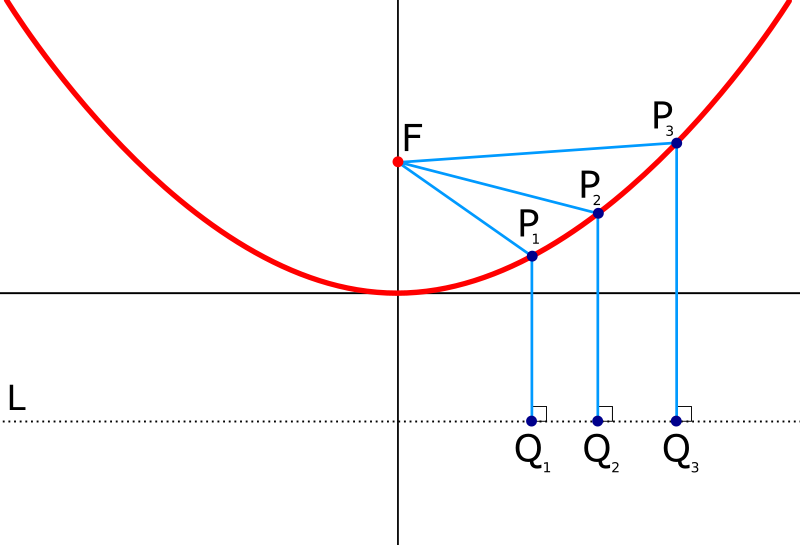
\includegraphics[scale=.3]{fig/parabola.png}
    \caption{Parabola with focus and directrix}
  \end{figure}
\end{frame}

\subsection{Screenshots}

\begin{frame}
  \frametitle{TODO}

  TODO

\end{frame}

\begin{frame}[plain]
  \itmobackgroundsnakes{
    \vfill
    \Huge{The End}
    \vfill
  }
\end{frame}

\end{document}
